\documentclass[colTwo]{NanouparIEEE}

 
% % % % % % % % % % % %
% Additional package
% % % % % % % % % % %
\usepackage{float}
\usepackage[siunitx]{circuitikz}



\begin{document}

    \researchgroup{NANOUPAR o Nombre de asignatura}
    
    \titlerunning{Título en español}
    \authorrunning{Rodríguez, Apellido y Apellido}
    % % % % % % % % % % % %
    \doi{www.github} % Link del PDF o codigo latex compartido
    % % % % % % % % % % % %
    \title{Título en espanol}
    
    \subtitle{English title} 
     	
     
    \author{Esteban A. Rodríguez M.\affilnum{1}, Nombre1 Nombre2 Apellido\affilnum{2} y Nombre1 Apellido\affilnum{3}}
    
    \affiliation{\affilnum{1} Estudiante de Ingeniería Mecatrónica, Escuela de pregrado de La Paz, Universidad Nacional de Colombia, Colombia. Afiliación: Estudiante. E-mail: esarodriguezme@unal.edu.co\\
    \affilnum{2} Abreviatura del Título Graduado o Actualmente estudiando, Institución, País. Títulos de Postgrado, Institución, País. Afiliación: Cargo actual, Institución, País. Correo electrónico: xxxx@xx.xx.xx \\
    \affilnum{2}Ingeniero Eléctrico, Universidad Nacional de Colombia, Colombia. M.Sc. Ingeniería Eléctrica, Universidad Nacional de Colombia, Colombia. Afiliación: Profesor asistente, Universidad Nacional de Colombia, Colombia. Correo electrónico: xxxx@xx.xx.xx}
    
    
    \begin{abstracts}
    \begin{abstract}[spanish]
    Lorem ipsum dolor sit amet, consectetur adipiscing elit. Etiam condimentum cursus dolor, quis pharetra enim hendrerit quis. Fusce et posuere dolor. Proin consequat faucibus magna, quis pellentesque lectus porttitor sit amet. Curabitur eu molestie diam. Morbi et lorem enim, et gravida est. Phasellus fringilla enim sed erat eleifend non pharetra erat vestibulum. In a sem leo. Cras in rutrum orci. Proin non quam sit amet lorem lobortis tincidunt eu vitae massa. Vivamus eros dui, porta non suscipit in, cursus in nulla. Nullam vitae hendrerit mi. Curabitur vehicula, metus a elementum luctus, augue sem ultricies turpis, vel lacinia diam purus eu tellus. Lorem ipsum dolor sit amet, consectetur adipiscing elit. Curabitur et mauris id ipsum consectetur semper. Pellentesque nec elit sit amet odio consequat mattis. Nunc placerat ultricies ullamcorper.
    \palwords{[PalabraClave1], [PalabraClave2], [PalabraClave3], [PalabraClave4].}
    \end{abstract}
    \begin{abstract}
    Lorem ipsum dolor sit amet, consectetur adipiscing elit. Etiam condimentum cursus dolor, quis pharetra enim hendrerit quis. Fusce et posuere dolor. Proin consequat faucibus magna, quis pellentesque lectus porttitor sit amet. Curabitur eu molestie diam. Morbi et lorem enim, et gravida est. Phasellus fringilla enim sed erat eleifend non pharetra erat vestibulum. In a sem leo. Cras in rutrum orci. Proin non quam sit amet lorem lobortis tincidunt eu vitae massa. Vivamus eros dui, porta non suscipit in, cursus in nulla. Nullam vitae hendrerit mi. Curabitur vehicula, metus a elementum luctus, augue sem ultricies turpis, vel lacinia diam purus eu tellus. Lorem ipsum dolor sit amet, consectetur adipiscing elit. Curabitur et mauris id ipsum consectetur semper. Pellentesque nec elit sit amet odio consequat mattis. Nunc placerat ultricies ullamcorper.
    \keywords{[Keyword1], [keyword2], [keyword3], [keyword4].}
    \end{abstract}
    %
    \end{abstracts}
    
    \maketitle
     

%%%%%%%%%%%%%%%%%%%%%% Begin the content %%%%%%%%%%%%%%%%%%%%%%


    \section{Introducción}
        \IEEEPARstart{S}{e} es libre de seleccionar y organizar el articulo de la mejor forma que usted crea combeniente para presentar su investigación/proyecto. Mas se considera que una estructura generalmente satisfactoria es:

        \begin{itemize}
            \item \textbf{Introducción}
            \item \textbf{Materiales y Métodos}
            \item \textbf{Resultados}
            \item \textbf{Discusión}
            \item \textbf{Apendice} (En caso de ser necesario)
            \item \textbf{Agradecimientos}
            \item \textbf{Bibliografia} (Obligatorio, Incluida por defecto)
        \end{itemize}

        A continuación, se encontraran diferentes secciones en donde se explica o se evidencian diferentes casos de uso que es posible se encuentre en la escritura de su trabajo.
        
        
	
    \section{Secciones}

        \subsection{Subsesion 1}
            Phasellus ante orci, accumsan vitae vulputate in, aliquam quis lacus. Aenean sit amet mauris quam, a semper velit. Maecenas feugiat sagittis felis eget mattis. Aenean bibendum porta orci, vitae lacinia turpis adipiscing a. 

        \subsection{Subsesion 2}
            Phasellus ante orci, accumsan vitae vulputate in, aliquam quis lacus. Aenean sit amet mauris quam, a semper velit. Maecenas feugiat sagittis felis eget mattis. Aenean bibendum porta orci, vitae lacinia turpis adipiscing a. 
            
            \subsubsection{Subsubsesion 1}
                Phasellus ante orci, accumsan vitae vulputate in, aliquam quis lacus. Aenean sit amet mauris quam, a semper velit. Maecenas feugiat sagittis felis eget mattis. Aenean bibendum porta orci, vitae lacinia turpis adipiscing a. 
            
            \subsubsection{Subsubsesion 2}
                Phasellus ante orci, accumsan vitae vulputate in, aliquam quis lacus. Aenean sit amet mauris quam, a semper velit. Maecenas feugiat sagittis felis eget mattis. Aenean bibendum porta orci, vitae lacinia turpis adipiscing a. 

        \subsection{Subsesion 3}
            Phasellus ante orci, accumsan vitae vulputate in, aliquam quis lacus. Aenean sit amet mauris quam, a semper velit. Maecenas feugiat sagittis felis eget mattis. Aenean bibendum porta orci, vitae lacinia turpis adipiscing a. 

    \section{Ecuaciones}

        \subsection{Normal}
            Phasellus ante orci, accumsan vitae vulputate in, aliquam quis lacus. Aenean sit amet mauris quam, a semper velit. Maecenas feugiat sagittis felis eget mattis. Aenean bibendum porta orci, vitae lacinia turpis adipiscing a. 

            \subsubsection{Sin numero de ecuación}
                Phasellus ante orci, accumsan vitae vulputate in, aliquam quis lacus. Aenean sit amet mauris quam, a semper velit. Maecenas feugiat sagittis felis eget mattis. Aenean bibendum porta orci, vitae lacinia turpis adipiscing a. 

                \begin{align*}
                    \overline{V_{geoC}} &= \frac{\sum_{i=1}^{3} \left(\frac{h_i \pi}{3} \left( (r_{1i})^2 + (r_{2i})^2 + (r_{1i})(r_{2i}) \right) \right)}{3}  \\
                    & = 7512.7603 \mathrm{mm^3} \\
                    & = 7.5127 \mathrm{ml}\\
                \end{align*}

            \subsubsection{Numero por linea}

                \begin{align}
                    \overline{V_{geoC}} &= \frac{\sum_{i=1}^{3} \left(\frac{h_i \pi}{3} \left( (r_{1i})^2 + (r_{2i})^2 + (r_{1i})(r_{2i}) \right) \right)}{3}  \\
                    & = 7512.7603 \mathrm{mm^3} \\
                    & = 7.5127 \mathrm{ml}\\
                \end{align}

            \subsubsection{Número en la ultima linea}

                \begin{align}
                    A \cdot \frac{d h_1}{d t} &= q_i-\frac{h_1-h_2}{r_1} \nonumber\\ 
                    \text{Multiplicando por } r_1 \nonumber\\
                    A_1 r_1 \frac{d h_1}{d t} &= q_t r_1-h_1+h_2\nonumber \\
                    A_1 r_1 &= \tau_1 \xrightarrow{} \text{Tiempo}\nonumber \\
                    \tau_1 \frac{d h_1}{dt}&= q_i r_1 -h_1 + h_2 \nonumber \\
                    \tau_1 \frac{d h_1}{dt} + h_1 &= q_i r_1 + h_2 \label{Eq.Num}
                \end{align}

        \subsection{Con texto}
            Phasellus ante orci, accumsan vitae vulputate in, aliquam quis lacus. Aenean sit amet mauris quam, a semper velit. Maecenas feugiat sagittis felis eget mattis. Aenean bibendum porta orci, vitae lacinia turpis adipiscing a. 
            
            \begin{align*}
                4000 \Omega \cdot I_1 - 2000 \Omega \cdot I_2 &= 4 \text{V} \quad \text{(Ec. 1)} \\
                8000 \Omega \cdot I_2 - 2000 \Omega \cdot I_1 &= 0 \quad \text{(Ec. 2)}
            \end{align*}

        \subsection{Multilinea}
            Phasellus ante orci, accumsan vitae vulputate in, aliquam quis lacus. Aenean sit amet mauris quam, a semper velit. Maecenas feugiat sagittis felis eget mattis. Aenean bibendum porta orci, vitae lacinia turpis adipiscing a. 
            
            \subsubsection{Forma 1}
                Phasellus ante orci, accumsan vitae vulputate in, aliquam quis lacus. Aenean sit amet mauris quam, a semper velit. Maecenas feugiat sagittis felis eget mattis. Aenean bibendum porta orci, vitae lacinia turpis adipiscing a. 
                
                \begin{multline*}
                    p_x = \frac{\cos{(t_1)}}{2} \cdot ( 125\cos{(t_2 + t_3 + t_4)} + 216\cos{(t_2 + t_3)} \\ + 180\cos{(t_2)} + 100)
                \end{multline*}
    
                \begin{multline*}
                    p_z = 145 - 108\sin{(t_2 + t_3)} - 90\sin{(t_2)} \\ - \frac{125\sin{(t_2 + t_3 + t_4)}}{2}
                \end{multline*}

            \subsubsection{Forma 2}
                Phasellus ante orci, accumsan vitae vulputate in, aliquam quis lacus. Aenean sit amet mauris quam, a semper velit. Maecenas feugiat sagittis felis eget mattis. Aenean bibendum porta orci, vitae lacinia turpis adipiscing a. 
                
                \begin{align*}
                    \begin{split}
                    m_1 &= \frac{125\cos{(t_2 + t_3 + t_4)}}{2} + 108\cos{(t_2 + t_3)} \\ 
                    & \quad \quad + 90\cos{(t_2)}
                    \end{split} \\
                    \begin{split}
                    m_2 &= \frac{125 \sin{(t_2 + t_3 + t_4)}}{2} + 108\sin{(t_2 + t_3)} \\ 
                    & \quad \quad + 90\sin{(t_2)}
                    \end{split}\\
                    m_3 &= 0 \\
                    n_1 &= p_x \cos{(t_1)} + p_y\sin{(t_1)} - 50 \\
                    n_2 &= 145 - p_z\\
                    n_3 &= p_y \cos{(t_1)} - p_x \sin{(t_1)}  
                \end{align*}
            

    \section{Matrices}

        Phasellus ante orci, accumsan vitae vulputate in, aliquam quis lacus. Aenean sit amet mauris quam, a semper velit. Maecenas feugiat sagittis felis eget mattis. Aenean bibendum porta orci, vitae lacinia turpis adipiscing a. 

        \subsection{Sin parentesis}
            Phasellus ante orci, accumsan vitae vulputate in, aliquam quis lacus. Aenean sit amet mauris quam, a semper velit. Maecenas feugiat sagittis felis eget mattis. Aenean bibendum porta orci, vitae lacinia turpis adipiscing a. 
            
            \begin{align}
                \begin{array}{lccl}
                \cos{\theta} & -\sin \theta * \cos \alpha & \sin \theta * \sin \alpha & a * \cos \theta \\
                \sin \theta & \cos \alpha * \cos \theta & -\cos \theta * \sin \alpha & a * \sin \theta \\
                0 & \sin \alpha & \cos \alpha & d \\
                0 & 0 & 0 & 1
                \end{array}
            \end{align}

        \subsection{Con parentesis}
            Phasellus ante orci, accumsan vitae vulputate in, aliquam quis lacus. Aenean sit amet mauris quam, a semper velit. Maecenas feugiat sagittis felis eget mattis. Aenean bibendum porta orci, vitae lacinia turpis adipiscing a. 
            
            \begin{align}
                \begin{pmatrix}
                    \cos{(t_1)} & 0 & -\sin{(t_1)} & 150\cos{(t_1)}\\
                    \sin{(t_1)} & 0 & \cos{(t_1)} & 150\sin{(t_1)} \\
                    0 & -1 & 0 & 400 \\
                    0 & 0 & 0 & 1\\
                \end{pmatrix}
            \end{align}
    
    \section{Imagenes}
        Phasellus ante orci, accumsan vitae vulputate in, aliquam quis lacus. Aenean sit amet mauris quam, a semper velit. Maecenas feugiat sagittis felis eget mattis. Aenean bibendum porta orci, vitae lacinia turpis adipiscing a. 
        
        \subsection{Una}
            Phasellus ante orci, accumsan vitae vulputate in, aliquam quis lacus. Aenean sit amet mauris quam, a semper velit. Maecenas feugiat sagittis felis eget mattis. Aenean bibendum porta orci, vitae lacinia turpis adipiscing a. 
            
            \begin{figure}[htbp]
                \centerline{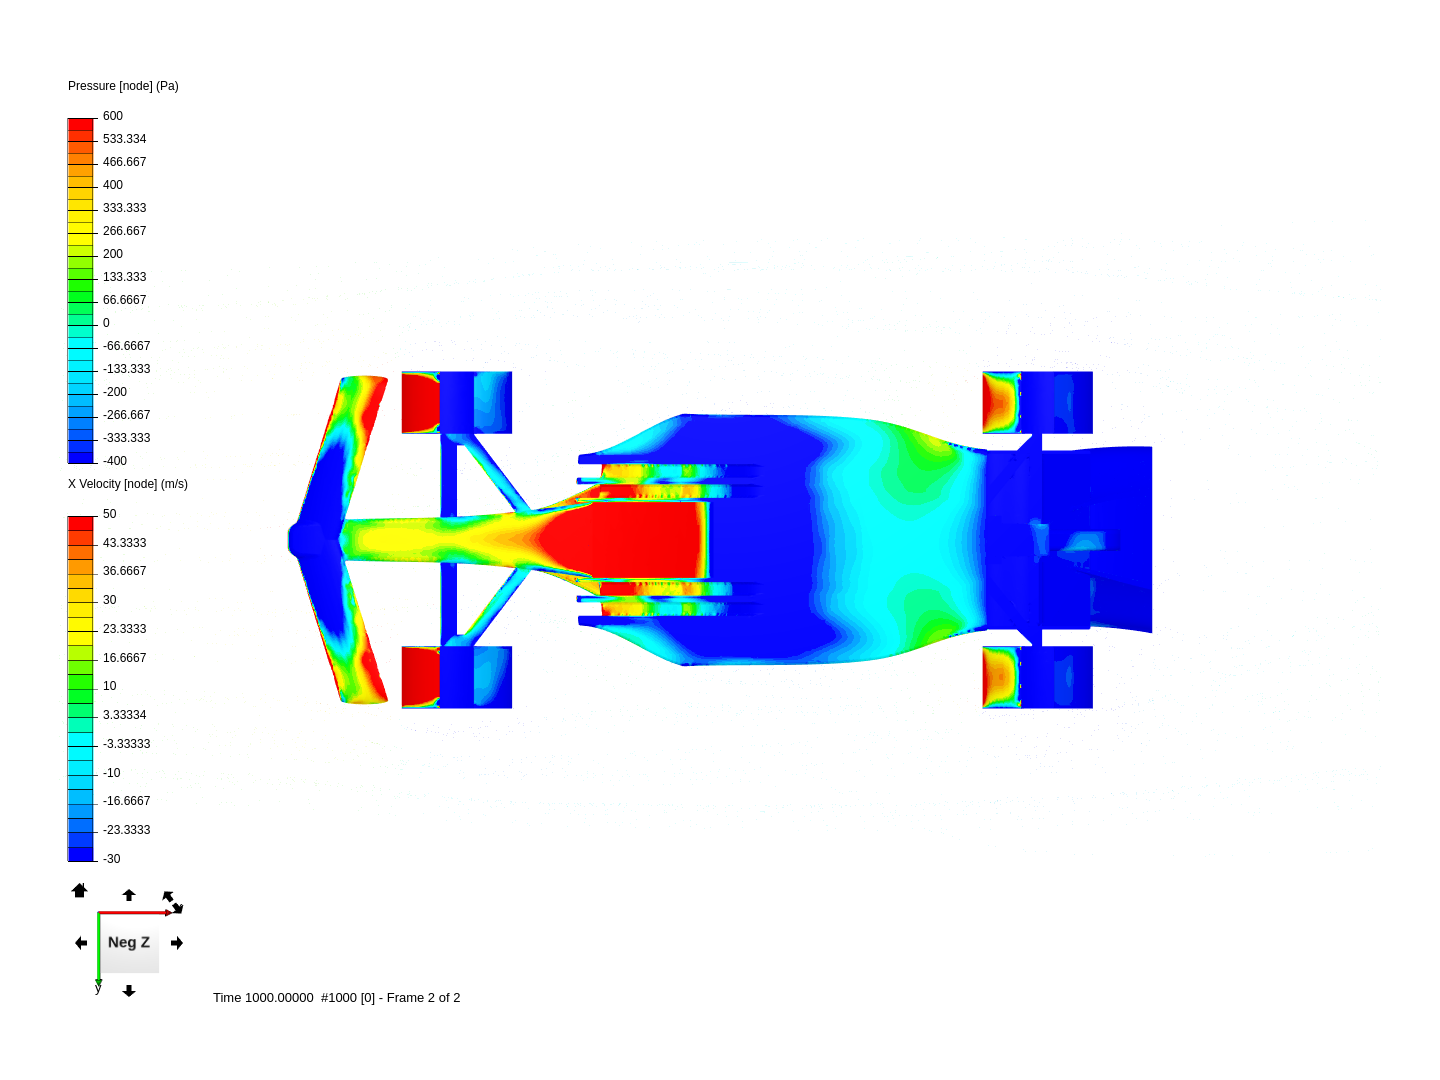
\includegraphics[scale=0.18]{images/Image_3-Inferior.png}}
                \caption{Presión en el vehículo, vista inferior.}
                \label{Fig.comportamiento_de_la_presion_inferior_vehiculo}
            \end{figure}

        \subsection{Cuatro}
            Phasellus ante orci, accumsan vitae vulputate in, aliquam quis lacus. Aenean sit amet mauris quam, a semper velit. Maecenas feugiat sagittis felis eget mattis. Aenean bibendum porta orci, vitae lacinia turpis adipiscing a. 

            \begin{figure}[htbp]
                \centering
                \begin{subfigure}[b]{0.235\textwidth}
                    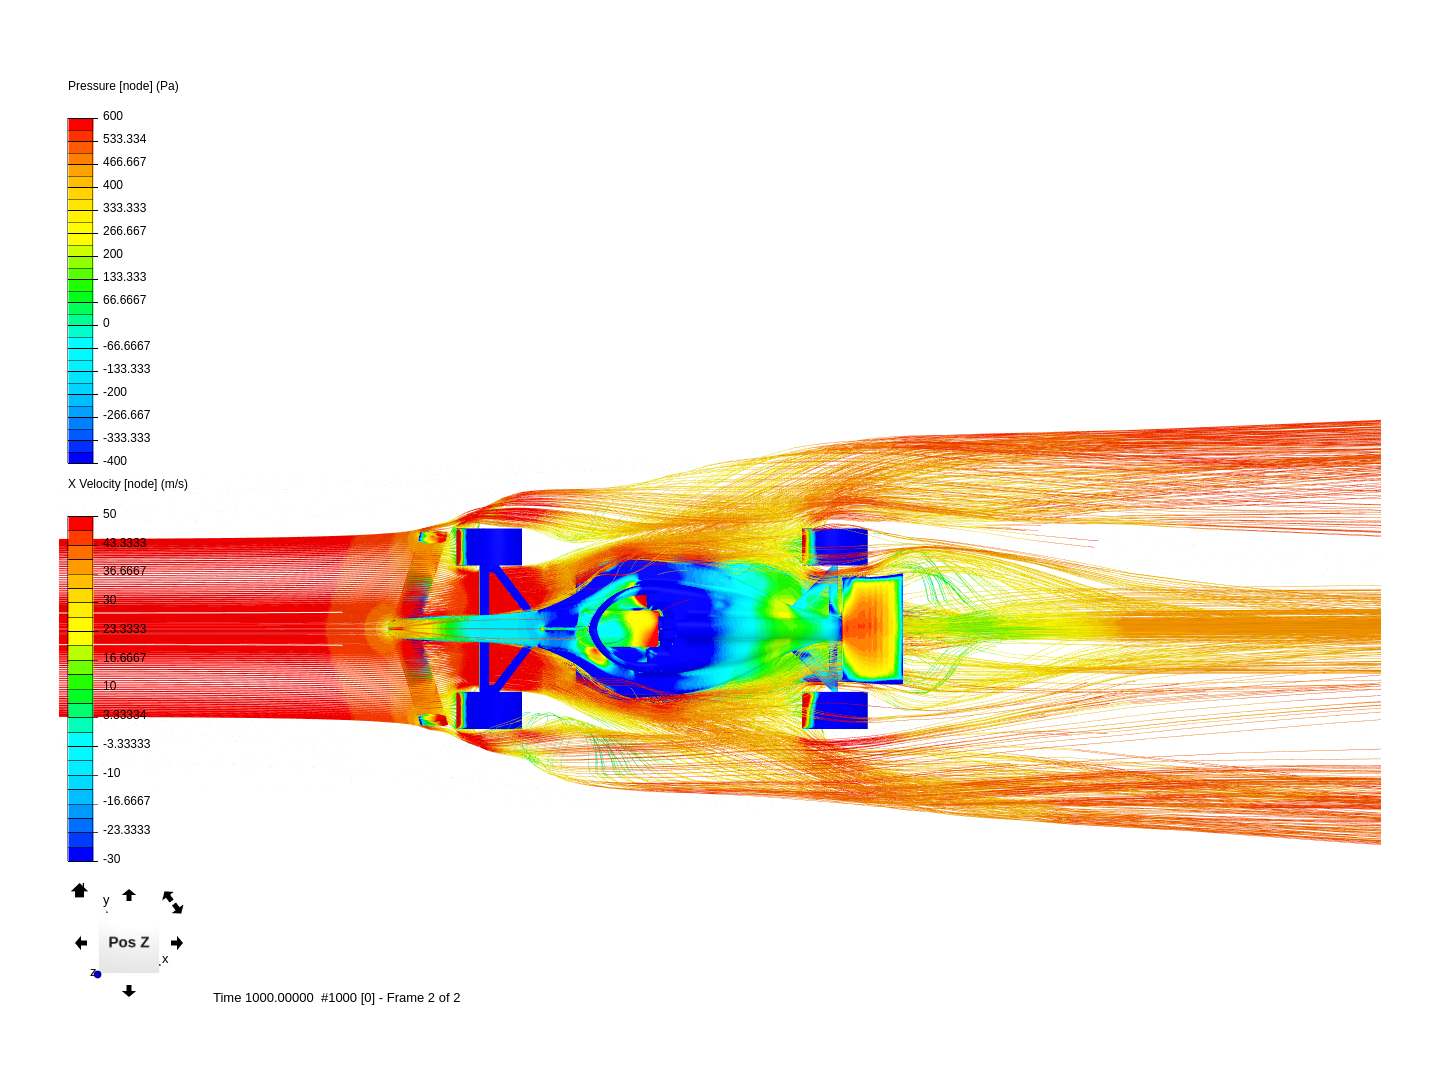
\includegraphics[width=\textwidth]{images/Image_5-Superior.png}
                    \caption{Vista superior}
                    \label{subFig.superior}
                \end{subfigure}
                \hfill
                \begin{subfigure}[b]{0.235\textwidth}
                    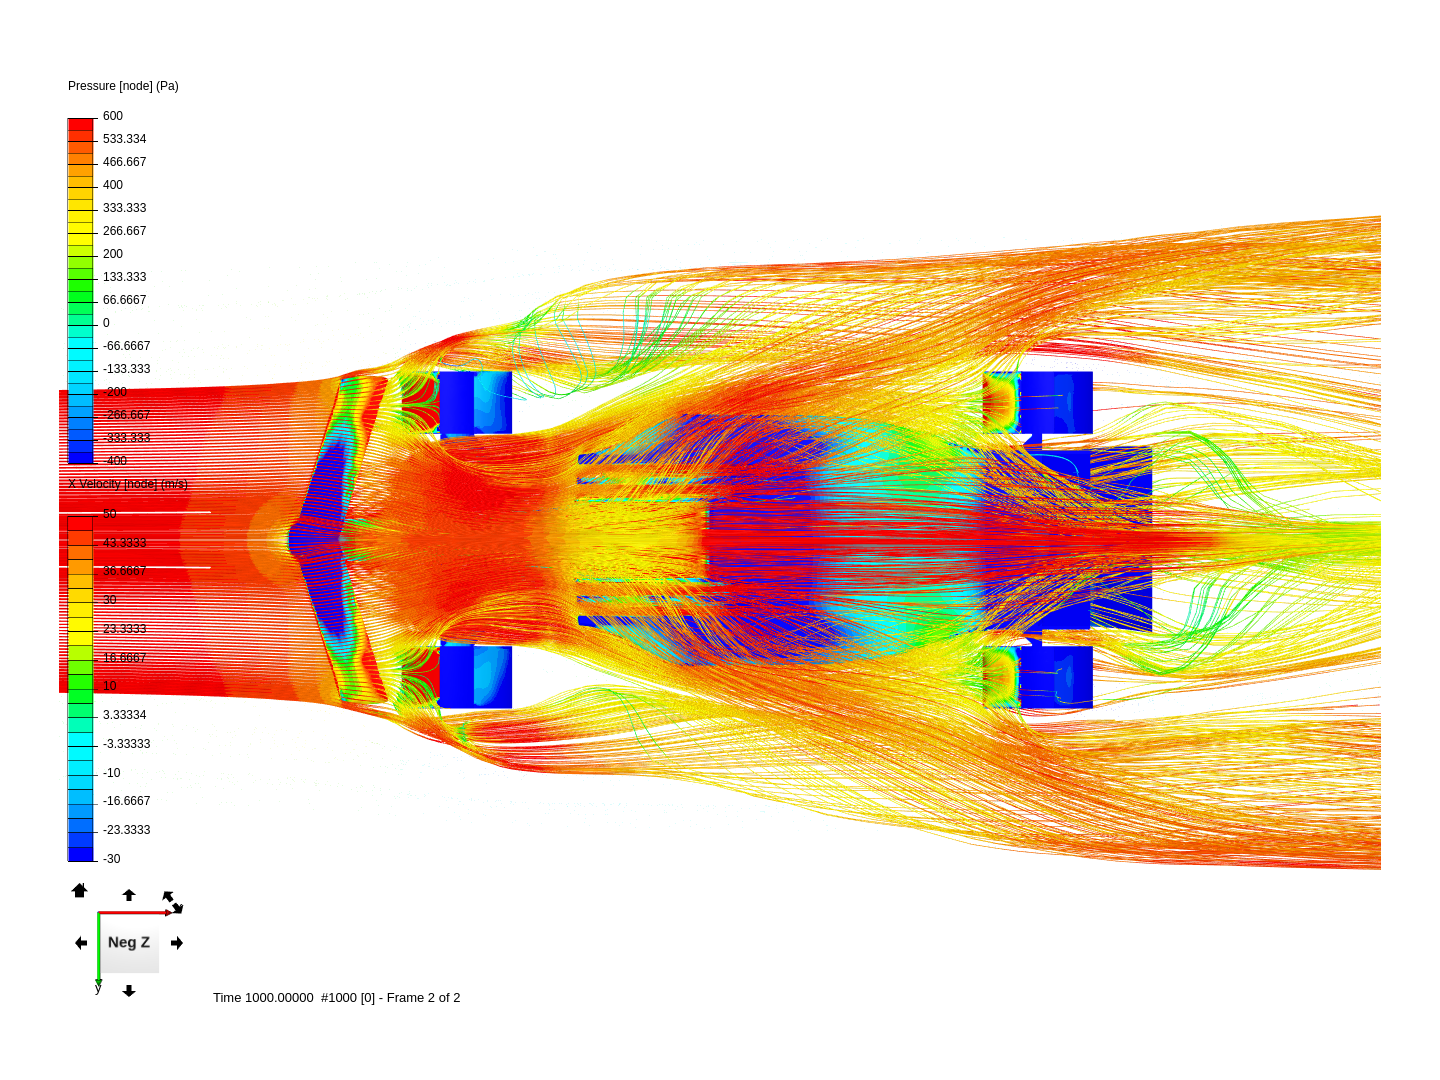
\includegraphics[width=\textwidth]{images/Image_6-Inferior.png}
                    \caption{Vista inferior}
                    \label{subFig.inferior}
                \end{subfigure}
                \\
                \begin{subfigure}[b]{0.235\textwidth}
                    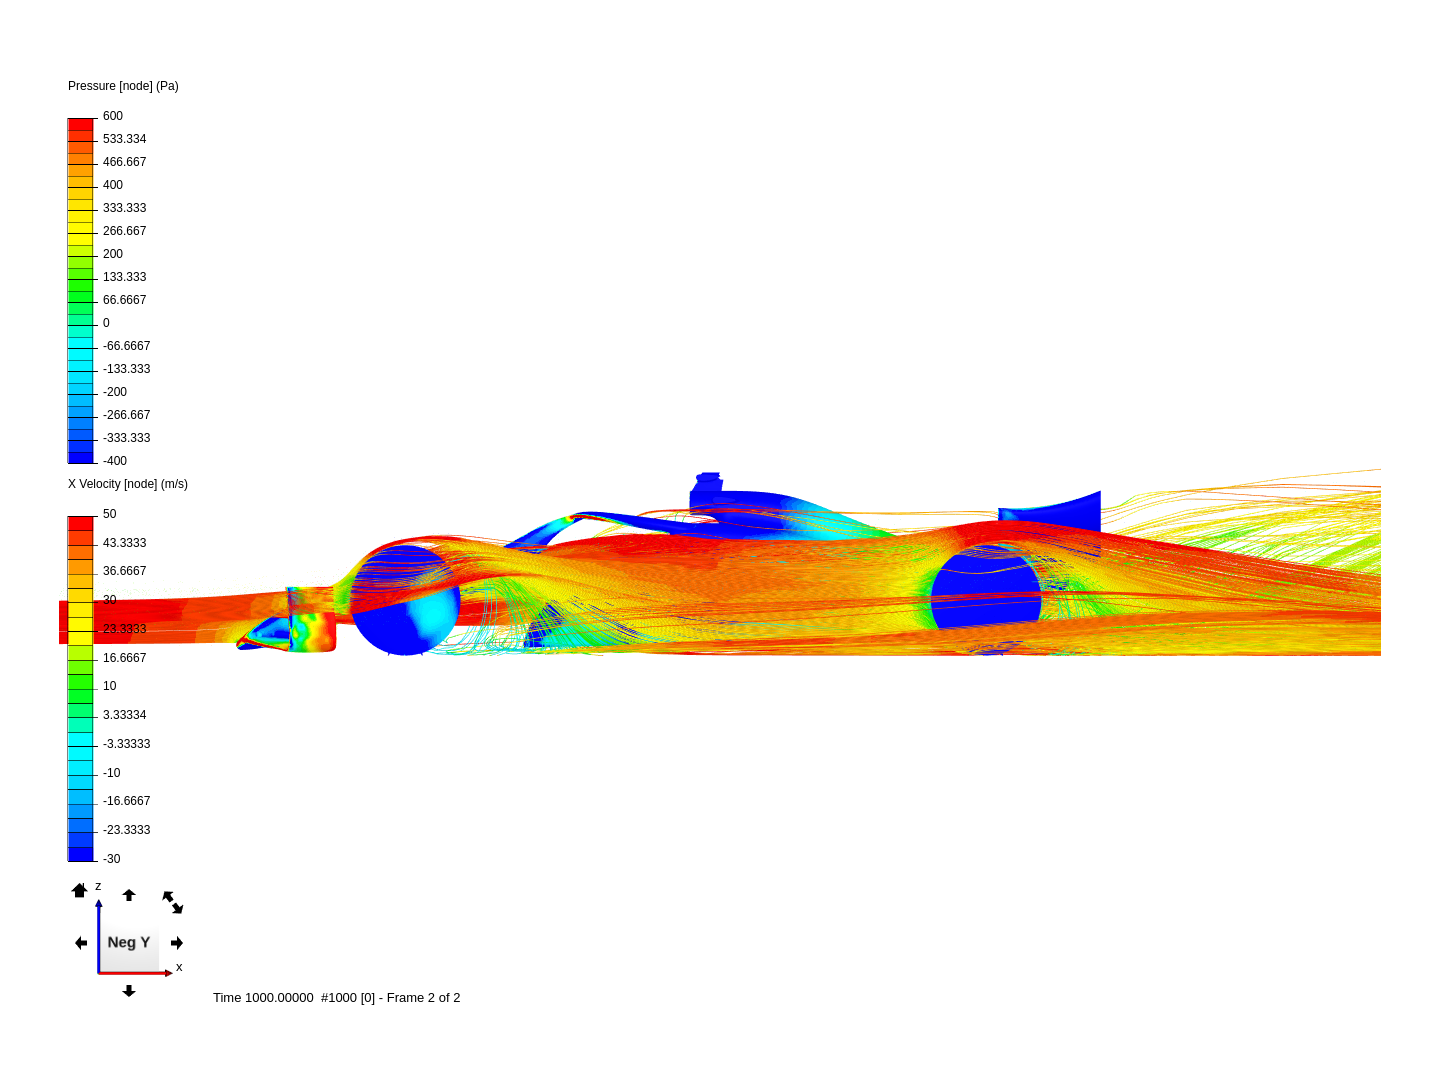
\includegraphics[width=\textwidth]{images/Image_7-Lateral.png}
                    \caption{Vista lateral}
                    \label{subFig.lateral}
                \end{subfigure}
                \hfill
                \begin{subfigure}[b]{0.235\textwidth}
                    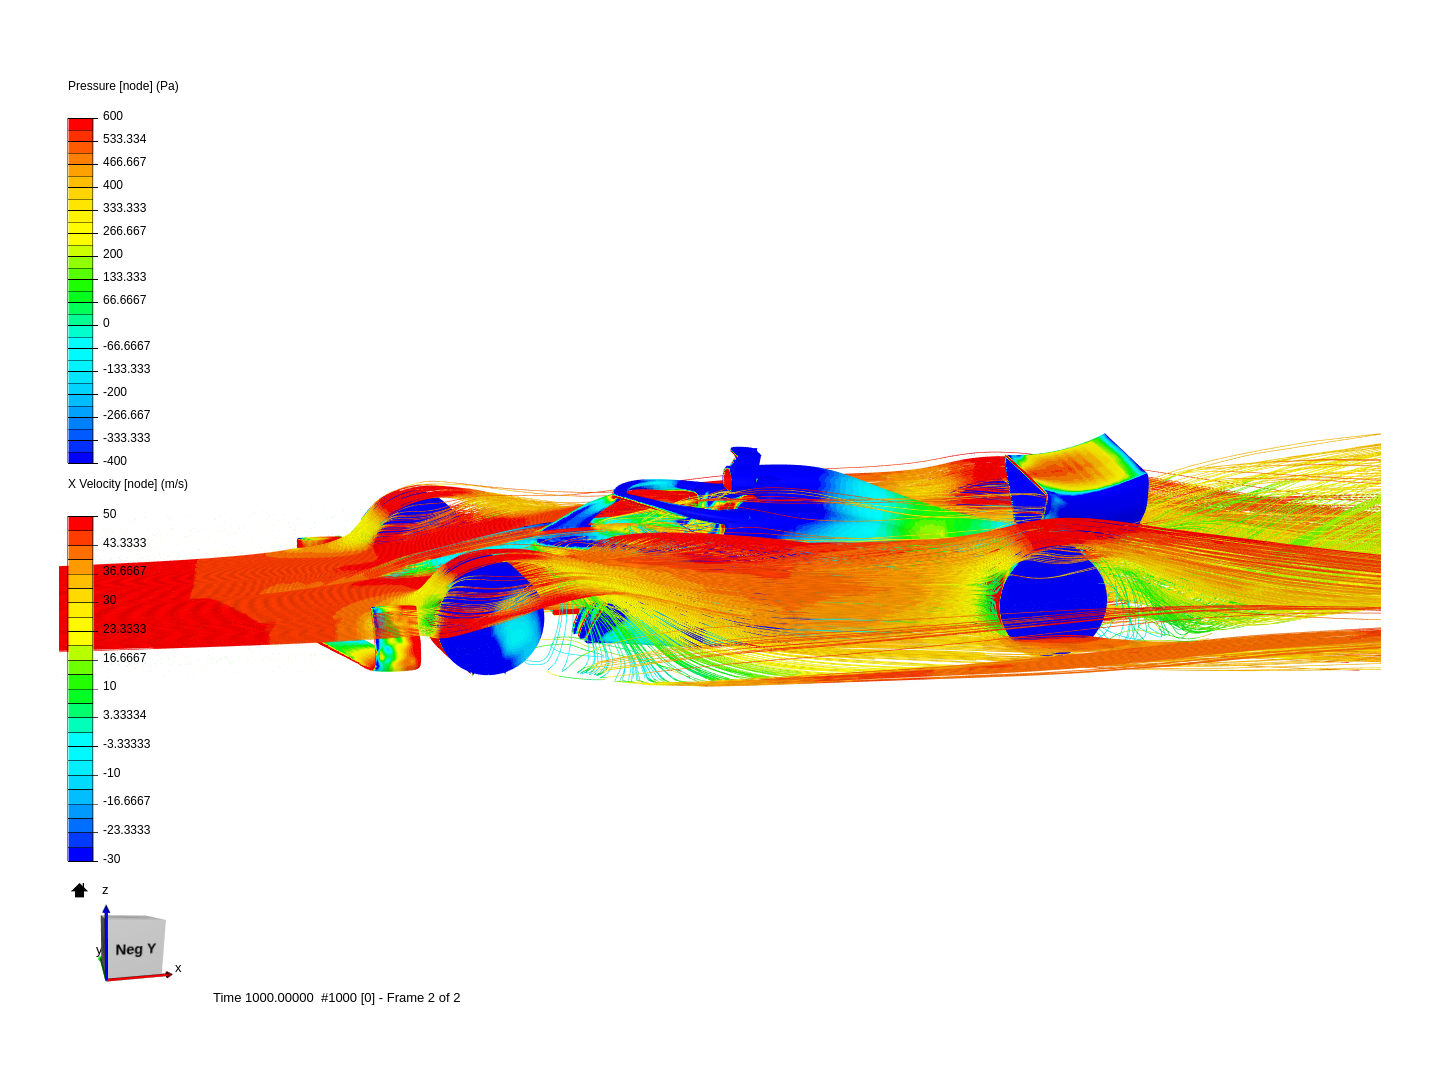
\includegraphics[width=\textwidth]{images/Image_8-Diagonal.png}
                    \caption{Vista diagonal}
                    \label{subFig.diagonal}
                \end{subfigure}
                \caption{Presión o fuerzas en el vehículo}
                \label{Fig.densidad_nodos_alta}
            \end{figure}

    \section{Tablas}

        \subsection{Normal}
            Phasellus ante orci, accumsan vitae vulputate in, aliquam quis lacus. Aenean sit amet mauris quam, a semper velit. Maecenas feugiat sagittis felis eget mattis. Aenean bibendum porta orci, vitae lacinia turpis adipiscing a. 

            \begin{table}[ht!]
                \caption{Medición de las longitudes características del corcho}
                \begin{center}
                    \begin{tabular}{l|c|c|c}
                        Muestra & Altura $(h)$ & Base inferior $(2r_1)$ & Base superior $(2r_2)$ \\
                        \hline \hline 
                        \# 1 & $23.17 \mathrm{mm}$ & $22.65 \mathrm{mm}$ & $17.86 \mathrm{mm}$\\
                        \hline 
                        \# 2 & $23.16 \mathrm{mm}$ & $22.68 \mathrm{mm}$ & $17.88 \mathrm{mm}$\\
                        \hline 
                        \# 3 & $23.19 \mathrm{mm}$ & $22.66 \mathrm{mm}$ & $17.89 \mathrm{mm}$\\
                        \hline
                        \end{tabular}
                \end{center}
                \label{medicion_longitudes_corcho}
            \end{table}

        \subsection{Anidadas}
            Phasellus ante orci, accumsan vitae vulputate in, aliquam quis lacus. Aenean sit amet mauris quam, a semper velit. Maecenas feugiat sagittis felis eget mattis. Aenean bibendum porta orci, vitae lacinia turpis adipiscing a. 
            
            \begin{table}[!htb]
                \centering\footnotesize\caption{Análisis de corriente}
                \begin{tabular}{lrr}
                    \multicolumn{3}{c}{\textbf{Corriente por $R_1$}}\\\hline
                    V & Teórico & Experimental \\\hline
                    $V_1$ & $\SI{10}{\milli\ampere}$ & $\SI{10.4}{\milli\ampere}$ \\\hline
                    $V_2$ & $\SI{20}{\milli\ampere}$ & $\SI{20.4}{\milli\ampere}$ \\\hline
                    $V_3$ & $\SI{30}{\milli\ampere}$ & $\SI{30.4}{\milli\ampere}$ \\\hline
                    $V_4$ & $\SI{40}{\milli\ampere}$ & $\SI{40.6}{\milli\ampere}$ \\\hline
                    $V_5$ & $\SI{50}{\milli\ampere}$ & $\SI{50.8}{\milli\ampere}$ \\\hline\hline
                \end{tabular}
                \begin{tabular}{lrr}
                    \multicolumn{3}{c}{\textbf{Corriente por $R_2$}}\\\hline
                    V & Teórico & Experimental \\\hline
                    $V_1$ & $\SI{0.1}{\milli\ampere}$ & $\SI{0.6}{\milli\ampere}$ \\\hline
                    $V_2$ & $\SI{0.2}{\milli\ampere}$ & $\SI{0.6}{\milli\ampere}$ \\\hline
                    $V_3$ & $\SI{0.3}{\milli\ampere}$ & $\SI{0.7}{\milli\ampere}$ \\\hline
                    $V_4$ & $\SI{0.4}{\milli\ampere}$ & $\SI{0.9}{\milli\ampere}$ \\\hline
                    $V_5$ & $\SI{0.5}{\milli\ampere}$ & $\SI{1.1}{\milli\ampere}$ \\\hline\hline
                \end{tabular}
                \begin{tabular}{lrr}
                    \multicolumn{3}{c}{\textbf{Corriente por $R_3$}}\\\hline
                    V & Teórico & Experimental \\\hline
                    $V_1$ & $\SI{2.1}{\milli\ampere}$ & $\SI{2.5}{\milli\ampere}$ \\\hline
                    $V_2$ & $\SI{4.3}{\milli\ampere}$ & $\SI{4.7}{\milli\ampere}$ \\\hline
                    $V_3$ & $\SI{6.4}{\milli\ampere}$ & $\SI{6.9}{\milli\ampere}$ \\\hline
                    $V_4$ & $\SI{8.5}{\milli\ampere}$ & $\SI{9}{\milli\ampere}$ \\\hline
                    $V_5$ & $\SI{10.6}{\milli\ampere}$ & $\SI{11.3}{\milli\ampere}$ \\\hline\hline
                \end{tabular}
            \end{table}

    \section{Circuitos electrónicos}

        Phasellus ante orci, accumsan vitae vulputate in, aliquam quis lacus. Aenean sit amet mauris quam, a semper velit. Maecenas feugiat sagittis felis eget mattis. Aenean bibendum porta orci, vitae lacinia turpis adipiscing a. Proin quis velit eu dolor auctor dapibus. Duis id nisi interdum quam scelerisque vestibulum sit amet et velit. Cum sociis natoque penatibus et magnis dis parturient montes, nascetur ridiculus mus. Donec odio leo, vulputate ut tempus in, malesuada in justo. Morbi commodo pharetra dapibus. In hac habitasse platea dictumst. Fusce sagittis ornare accumsan. Vivamus scelerisque, arcu tempor pulvinar convallis, lectus nisl condimentum velit, eget cursus magna eros imperdiet purus. Maecenas a vehicula tortor.

        \begin{center}
            \begin{circuitikz}[american voltages, american currents]
                \draw[red] 
                (0,0) to [short,-] (0,-0.5)
                (0,-1.5) to [short,-] (0,-2)
                (0,-2) to [short,-] (4,-2)
                (4,-2) to [short,-] (4,0)
                (3,0) to [short,-] (2.5,0)
                (1.5,0) to [short,-] (0,0);
                \draw
                (0,-0.5) to [V, l^=${}^{V_4}_{10V}$] (0,-1.5)                        
                (2.5,0) to [R, l^=${}^{R_4}_{220\mathrm{\Omega}}$] (1.5,0)
                (2,-2) node [ground]{};

                \draw [red]
                (3,0) to [short,-] (4,0);
            \end{circuitikz}
        \end{center}

        Phasellus ante orci, accumsan vitae vulputate in, aliquam quis lacus. Aenean sit amet mauris quam, a semper velit. Maecenas feugiat sagittis felis eget mattis.

        \begin{center}
            \begin{circuitikz}[american voltages, american currents]
                \draw[red] 
                (0,0) to [short,-] (0,-0.5)
                (0,-1.5) to [short,-] (0,-2)
                (0,-2) to [short,-] (4,-2)
                (4,-2) to [short,-] (4,0)
                (3,0) to [short,-] (2.5,0)
                (1.5,0) to [short,-] (0,0);
                \draw
                (0,-0.5) to [V, l^=${V_6}$] (0,-1.5)                        
                (2.5,0) to [R, l^=${}^{R_6}_{5\mathrm{\Omega}}$] (1.5,0)
                (2,-2) node [ground]{};

                \draw[blue] 
                (3,0) to [short,i^=$1\mathrm{mA}$] (4,0);
            \end{circuitikz}
        \end{center}

        Phasellus ante orci, accumsan vitae vulputate in, aliquam quis lacus. Aenean sit amet mauris quam, a semper velit. Maecenas feugiat sagittis felis eget mattis.

        \begin{center}
            \begin{circuitikz}[american voltages, american currents]
                \draw 
                (0,0) to [short,-] (0,-0.5)
                (0,-1.5) to [short,-] (0,-2)
                (0,-2) to [short,-] (4,-2)
                (5,-2) to [short,-] (6,-2)
                (6,-2) to [short,-] (6,-1.5)
                (6,-0.5) to [short,-] (6,0)
                (6,0) to [short,-] (5,0)
                (4,0) to [short,-] (3,0)
                (2,0) to [short,-] (0,0)
                (0,-0.5) to [V, l^=${}^{V_8}_{15V}$] (0,-1.5)
                (3,0) to [R, l_=${}^{R_8}_{5.8\mathrm{k\Omega}}$] (2,0)
                (5,0) to [R, l_=${}^{R_9}_{18\mathrm{k\Omega}}$] (4,0)
                (6,-1.5) to [R, l_=${}^{R_{10}}_{56\mathrm{k\Omega}}$] (6,-0.5)
                (4,-2) to [R, l_=${}^{R_{11}}_{22\mathrm{k\Omega}}$] (5,-2)
                
                (2,-2) node [ground]{};

            \end{circuitikz}
        \end{center}

        Phasellus ante orci, accumsan vitae vulputate in, aliquam quis lacus. Aenean sit amet mauris quam, a semper velit. Maecenas feugiat sagittis felis eget mattis.

        \begin{center}
            \begin{circuitikz}[american voltages, american currents]
                \draw
                (0,0) to [V=${V_S}$,invert, *-] (0,2) -- (0,4)
                to[R=$R_1$] node[pos=0.05,below left=1.25ex] {$P_1$} (6,4) -- (6,0) -* (0,0)
                (0,2) to[R=$R_1$, *-*] node[pos=0.05,below left=1.25ex] {$P_2 =$\SI{0.75}{\kilo\watt}} (6,2)

                (4.5,3.75) to [short,i_=$I_1$] (5.5,3.75)
                (4.5,1.75) to [short,i_=$I_2$] (5.5,1.75)
                (3.5,-0.25) to [short,i^=\SI{200}{\milli\ampere}] (2.5,-0.25)

                (3,0.25) node {$P_T = \SI{2}{\watt}$}
                
                (0,0) node [ground]{};

            \end{circuitikz}
        \end{center}

        Phasellus ante orci, accumsan vitae vulputate in, aliquam quis lacus. Aenean sit amet mauris quam, a semper velit. Maecenas feugiat sagittis felis eget mattis.

        \begin{center}
            \begin{circuitikz}[american voltages, american currents]
                \draw
                (0,0) to [R, l_=$3\mathrm{k\Omega}$] (0,-4)
                to [short, -*] (2.5,-4)
                to [short, -*] (5,-4)
                to [short, -] (6.5,-4)
                to [R, l_=$2\mathrm{k\Omega}$] (6.5,0)
                to [short, -*] (5,0)
                to [R, l_=$2\mathrm{k\Omega}$] (2.5,0)
                to [short, *-] (0,0)
                
                (0.5,0) to [open, v^>=$V_1$] (0.5,-4)
                (2.5,0) to [I, l_=$6\mathrm{mA}$] (2.5,-4)
                
                (5,0) to [I, l^=$4\mathrm{mA}$] (2.5,-4)
                (5,0) to [R, l^=$2\mathrm{k\Omega}$] (5,-4);
            \end{circuitikz}
        \end{center}

        Phasellus ante orci, accumsan vitae vulputate in, aliquam quis lacus. Aenean sit amet mauris quam, a semper velit. Maecenas feugiat sagittis felis eget mattis.

        \begin{center}
            \begin{circuitikz}[american voltages, american currents]
                \draw
                (0,0) to [R, l_=$2\mathrm{k\Omega}$] (0,-4)
                to [short, -*] (2.5,-4)
                to [short, -*] (5,-4)
                to [short, -] (7,-4)
                to [open,o-o] (7,0)
                to [short, -*] (5,0)
                to [V, l_=$12\mathrm{V}$, -*] (2.5,0)
                
                (0,0) to [V, l^=$6\mathrm{V}$] (2.5,0)

                (7,0) to [open,v_=$V_0$] (7,-4)
                
                (2.5,0) to [R, l_=$4\mathrm{k\Omega}$] (2.5,-4)
                
                (5,0) to [R, l^=$2\mathrm{k\Omega}$] (5,-4);
                
                \draw[orange,thick,dashed] (4.5,0.25) -- (4.5,-4.25);
                \draw (4.5,0.25) node[anchor=west] {\textbf{A}};
                \draw (4.5,-4.25) node[anchor=west] {\textbf{B}};
                
            \end{circuitikz}
        \end{center}

        Phasellus ante orci, accumsan vitae vulputate in, aliquam quis lacus. Aenean sit amet mauris quam, a semper velit. Maecenas feugiat sagittis felis eget mattis.

         \begin{center}
            \begin{circuitikz}[american voltages, american currents]
                \draw
                (0,0) to [V, l^=$20\mathrm{V}$] (0,-6)
                to [short, -] (7,-6)
                to [open, *-*] (7,0)
                to [R, l_=$50\mathrm{\Omega}$] (5,0)
                to [R, l_=$24\mathrm{\Omega}$] (2.5,0)
                to [R, l_=$80\mathrm{\Omega}$] (0,0)
                
                (2.5,0) to [R, l^=$25\mathrm{\Omega}$] (2.5,-3)
                (1.75,-3) to [short,-](3.25,-3)
                (1.75,-3) to [R, l_=$60\mathrm{\Omega}$] (1.75,-6)
                (3.25,-3) to [R, l^=$20\mathrm{\Omega}$] (3.25,-6)
                
                (5,0) to [R, l^=$20\mathrm{\Omega}$] (5,-6)
                
                (7,-2) to [open,v_=$V_{TH}$] (7,-4);

                \draw [<-] (2,-2) arc (0:75:1);
                \draw [<-] (2.8,-5) arc (0:75:1);
                \draw [<-] (4.25,-2) arc (0:75:1);

                \draw (2,-2) node[anchor=east] {$I_1$};
                \draw (2.8,-5) node[anchor=east] {$I_2$};
                \draw (4.25,-2) node[anchor=east] {$I_3$};
                % \draw [->](0,-2) to (1,-2);
                
            \end{circuitikz}
        \end{center}

    \section{Referencias entre el documento}

        Se selecciona el perfil de impresión \textit{Normal Quality} que se encuentra por defecto en el software, sobreescribiendo los valores de las características que se listan por los incluidos en la tabla \ref{parametros_impresion}.
        \begin{table}[ht!]
            \caption{Parámetros generales de impresión}
            \begin{center}
                \begin{tabular}{l|r}
                    Profile settings & Customized \\
                    \hline \hline \multicolumn{2}{c}{\textbf{Dual Extrusion}} \\
                    \hline Prime Tower X Position & $230$ \\
                    \hline Prime Tower Y Position & $213.6$ \\
                    \hline \hline \multicolumn{2}{c}{\textbf{Support}} \\ 
                    \hline Generate Support & False \\
                    \hline \hline \multicolumn{2}{c}{\textbf{ Build Plate Adhesion}} \\ 
                    \hline Build Plate Adhesion Type & skirt\\
                    \hline Skirt Line Count (Extruder) & 2 \\
                    \hline \hline \multicolumn{2}{c}{\textbf{Travel}} \\ 
                    \hline Combing Mode & all \\
                    \hline \hline \multicolumn{2}{c}{\textbf{Infill}} \\ 
                    \hline Infill Before Walls (Extruder) & True \\
                    \hline Infill Density (Extruder) & \textit{Varios} \\
                    \hline
                    \end{tabular}
            \end{center}
            \label{parametros_impresion}
        \end{table}
            

    \section{Citas}

        Para citar, debe añadir la cita en formato bibtex en el documento \textbf{bibtex $>$ IEEEbiblio.bib} y citarlo como se encuentra en el siguiente parrafo.

        El uso de la nanotecnología en el campo de la medicina ha mejorado los procesos en el diagnóstico y tratamiento que requieren una intervención cuidadosa y precisa, por su facilidad en la penetración de barreras biológicas \cite{01_nano_in_medicine}, además de un progreso en la duración de la vida útil de fármacos que tienen impacto en enfermedades crónicas, reduciendo su degradación luego de haber ingresado al organismo \cite{han2021emerging}\cite{el2020advances}, enfrentando uno de los retos en los sistemas de administración de medicamentos \cite{homayun2019challenges}.

    \bibliography{bibtex/ref.bib}
    \bibliographystyle{IEEEtran}
    

\end{document}